\documentclass[conference]{IEEEtran}

\IEEEoverridecommandlockouts
% The preceding line is only needed to identify funding in the first footnote. If that is unneeded, please comment it out.
\usepackage{cite}
\usepackage{amsmath,amssymb,amsfonts}
\usepackage{algorithm}
\usepackage{graphicx}
\usepackage{textcomp}
\usepackage{xcolor}
\usepackage{CJKutf8}
\usepackage{algpseudocode}
\usepackage{hyperref}
\def\BibTeX{{\rm B\kern-.05em{\sc i\kern-.025em b}\kern-.08em
    T\kern-.1667em\lower.7ex\hbox{E}\kern-.125emX}}
\begin{document}
\begin{CJK*}{UTF8}{bsmi}

\title{Spectral Efficiency Analysis of Uplink-Downlink Decoupled Access in C-V2X Networks\\
{\normalsize {PERFORMANCE MODELING FOR MOBILE COMMUNICATIONS NETWORKING SYSTEMS FINAL PROJECT}}}

\author{
\IEEEauthorblockN{徐振宗}
\IEEEauthorblockA{資工所碩一\ r11922188}\\
\and
\IEEEauthorblockN{栗漢文}
\IEEEauthorblockA{資工所碩一\ r11922191}\\
\and
\IEEEauthorblockN{青光恆}
\IEEEauthorblockA{資工所碩一\ r11922120}\\
}

\maketitle

\begin{abstract}
With the development of mobile networks, C-V2X applications are becoming more and more advanced. We studied a paper on how to establish an analysis model for C-V2X and simulated to reproduce the experimental results of this paper.
\end{abstract}
\section{Introduction}
\par 3GPP Cellular V2X (C-V2X) is an innovative technology designed for transportation that allows cars to communicate with each other and even with surrounding devices. In order to improve the safety of drivers, passengers and pedestrians, C-V2X provides low-latency communication directly between general vehicles (V2V), roadside infrastructure (V2I), drivers and pedestrians (V2P), and cars to the network (V2N). Therefore, the quality of service (QoS) of the network is important for C-V2X applications. 
\par Currently, C-V2X is gradually evolving into a more complex heterogeneous network composed of macro base stations (MBS) and small base stations (SBS). It is generally believed that users located at the edge of SBS choose to access SBS in uplink (UL) and MBS in downlink (DL), which can significantly improve the UL rate in heterogeneous networks in cellular networks. This is essential for high UL rate guarantees such as safety information sharing and remote driving in C-V2X. 
\par Therefore, the paper we found studies the spectrum efficiency of UL and DL access to different base stations in C-V2X. It models UL/DL decoupling access to C-V2X as a Cox process and proposes a unified analytical framework. Through stochastic geometry, it provides in-depth theoretical analysis, including joint association probability, UL/DL distance distribution to service BS, and associated cases in C-V2X networks.


\section{System Model}
The system model consists of the following five elements (\autoref{Fig:model}): 
\begin{itemize}
    \item[]
    \begin{itemize}
        \item The overall area of the system 
        \item Macro Base Station (MBS)
        \item Road 
        \item Small Base Station (SBS) 
        \item Vehicle
    \end{itemize}
\end{itemize}

\begin{figure}[htbp]
\centering
\includegraphics[scale=0.25]{model.eps}
\caption{\label{Fig:model}Illustration of the system model}
\end{figure}

\begin{enumerate}
    \item The overall area of the system is set as a plane of a circle with a radius of R.
    \item Macro Base Station (MBS) is evenly distributed in the circle and simulated using a 2D Poisson point process (PPP) with a density $\lambda_m$.
    \\
    \item Roads are simulated by Poisson Line process (PLP). In the plane, lines can be transformed into a 1-to-1 transformation by taking the intersection of the perpendicular line from the origin to the line. And then transform the point into polar coordinates (\autoref{Fig:PLP}). Therefore, we can use 2D PPP to simulate PLP, and the density of PPP is  $\lambda_r$.
    \\
    \item Small Base Station (SBS) is simulated using a 1D PPP with density $\lambda_s$ on each line generated by 3.
    \\
    \item Vehicle is simulated using a 1D PPP with a density $\lambda_v$ on each line generated by 3.
\end{enumerate}

\begin{figure}[htbp]
\centering
\includegraphics[scale=0.2]{PLP.eps}
\caption{\label{Fig:PLP}Illustration of a line converted into point\cite{b2}}
\end{figure}

%栗begin
\subsection{Power Transmission}
To analyze the transmission power between vehicles and base stations (BS) in this model, this paper defines the following transmission powers:\\
the DL transmit power can be written as
$$
\begin{aligned}
P_{r, V}=
\begin{cases}
P_M G_M H_M \chi_M\|x\|^{-\alpha_M}, & x \in \Phi_M \\
P_S G_{S, 0} H_{S, 0} \chi_{S, 0}\|x\|^{-\alpha_S}, & x \in \Xi_{l_0}^{(S)} \\
P_S G_{S, 1} H_{S, 1} \chi_{S, 1}\|x\|^{-\alpha_S}, & x \in \Phi_S \backslash \Xi_{l_0}^{(S)},
\end{cases}
\end{aligned}
$$
the UL transmit power can be written as
$$
\begin{aligned}
P_{r, M}=P_V G_{V, 1} H_{V, 1} \chi_M\|x\|^{-\alpha_M}, \quad x \in \Phi_M \text {, } \\
P_{r, S}= \begin{cases}P_V G_{V, 0} H_{V, 0} \chi_{S, 0}\|x\|^{-\alpha_S}, & x \in \Xi_{l_0}^{(S)} \\
P_V G_{V, 1} H_{V, 1} \chi_{S, 1}\|x\|^{-\alpha_S}, & x \in \Phi_S \backslash \Xi_{l_0}^{(S)},\end{cases} \\
\end{aligned}\\
$$

and the definition of parameters above are as follows.
$$
\begin{aligned}
&\Phi_M: \text {the set of MBSs}\\
&\Phi_S:  \text {the set of SBSs}\\
&\Xi_{l_0}^{(S)}: \text {the set of SBSs in the typical line}\\
&P: \text {transmit power}\\
&G: \text {antenna gains}\\
&H: \text {channel fading gains}\\
&\chi: \text {shadowing effects}\\
&x: \text {distance between vehicle and BS}\\
&\alpha: \text {power-law loss parameters}
\end{aligned}
$$
These three power measurements are further categorized into different cases based on the type of base station.  The \autoref{fig:power_cases} shows the cases in different base station applied scenarios.\\

\begin{figure}[htbp]
\centering
\includegraphics[scale=0.50]{power_cases.png}
\caption{\label{fig:power_cases}Power transmission between different base station}
\end{figure}

\subsection{Power Transmission Cases}
For the convenience of analysis, this paper divides the cases based on the base stations (BS) connected to the downlink (DL) and uplink (UL) into four categories as follows.
\begin{itemize}
    \item[]
    \begin{itemize}
        \item Case 1: UL = MBS, DL = MBS
        \item Case 2: UL = SBS, DL = MBS
        \item Case 3: UL = MBS, DL = SBS
        \item Case 4: UL = SBS, DL = SBS
    \end{itemize}
\end{itemize}

%栗end

%光
\section{Spectral Efficiency Analysis}
We assume that a vehicle is associated with the MBS/SBS which yields the highest biased received power in DL, similarly,the MBS/SBS will serve the vehicle with the highest transmit power in UL, namely the vehicles in the Voronoi cell of a BS connect to it.
\par Spectral efficiency refers to the amount of data that can be transmitted over a given bandwidth. In this paper, summing up the data rates in different cases yields our Spectral Efficiency.


\subsection{Distance Distribution}

we first need to compute the distance distribution between the vehicle and the BS. the cumulative distribution functions (CDF) of $x_S, x_M$ are

\begin{equation}
\begin{aligned}
F_S(x_S)=1-\exp(-2\lambda_S x_S)\\
F_S(x_S)=1-\exp(-\lambda_M \pi x_S^2)
\end{aligned}
\end{equation}


According to $f(x) = dF(x)/dx$, the probability density
functions (PDF) of $x_S, x_M$ are

\begin{equation}
\begin{aligned}
f_S\left(x_S\right) & =2 \lambda_S \exp \left(-2 \lambda_S x_S\right) \\
f_M\left(x_M\right) & =2 \pi x_M \lambda_M \exp \left(-\lambda_M \pi x_M^2\right)
\end{aligned}
\end{equation}


\subsection{Joint Association Probability}

Since both UL and DL are connected to MBS in Case 1, we can derive the following formula:

\begin{equation}
\begin{aligned}
P_M G_M B_M\left\|x_M\right\|^{-\alpha_M}>P_S G_{S, 0} B_S\left\|x_S\right\|^{-\alpha_S} \\
P_V G_{V, 1}\left\|x_M\right\|^{-\alpha_M}>P_V G_{V, 0}\left\|x_S\right\|^{-\alpha_S}
\end{aligned}
\end{equation}
We denote
\begin{equation}
\begin{aligned}
A_{M, S}=P_M G_M B_M / P_s G_{s, 0} B_s \\
B_{M, S}=P_V G_{V, 1} / P_V G_{V, 0}\\
\end{aligned}
\end{equation} \\

Substituting for $(3)$ :

\begin{equation}
\begin{aligned}
A_{M, S}\left\|x_M\right\|^{-\alpha_M}>\left\|x_S\right\|^{-\alpha_S},\\
B_{M, S}\left\|x_M\right\|^{-\alpha_M}>\left\|x_S\right\|^{-\alpha_S},
\end{aligned}
\end{equation}
%
Furthermore, since the transmit power of MBS is much larger than that of SBS and vehicle, we can assume that $A_{M, S}> B_{M, S}$.So the joint probability of Case 1 can be written as:
\begin{equation}
\begin{aligned}
&\operatorname{Pr}(\text {Case} 1)=\operatorname{Pr}(A_{M, S} X_M^{-\alpha_M}>X_S^{-\alpha_S} ;B_{M, S} X_M^{-\alpha_M}>X_S^{-\alpha_S}) \\
&=\operatorname{Pr}\left(B_{M, S} X_M^{-\alpha_M}>X_S^{-\alpha_S}\right) \\
&=E_{X_S}\left[\operatorname{Pr}\left(X_M<B_{M, S}^{\frac{1}{\alpha_M}} x_S^{\frac{\alpha_S}{\alpha_M}} \mid X_S\right)\right] \\
&=\int_0^{\infty} F_M\left(B_{M, S}^{\frac{1}{\alpha M}} x_S^{\frac{\alpha_S}{\alpha_M}}\right) f_S\left(x_S\right) d x_S \\
& = 1-\int_0^{\infty}\left[2 \lambda_S \exp \left(-\lambda_M \pi B_{M, S}^{\frac{2}{\alpha_M}} x_S^{\frac{2 \alpha_S}{\alpha_M}}-2 \lambda_S x_S\right)\right] d x_S, \\
\end{aligned}
\end{equation}
Since $x_S$ and $x_M$ are both random variables, we can consider this as the summation of the probability that $x_M$ satisfies the condition for different $x_S$. Then, by applying the derived CDF and PDF formulas for distance, we can obtain the probability of each case occurring.

\begin{equation}
\begin{aligned}
&\operatorname{Pr}(\text { Case } 2)=\operatorname{Pr}\left(A_{M, S} X_M^{-\alpha_M}>X_S^{-\alpha_S} ;\right. \\
&\qquad\qquad\qquad \left.B_{M, S}X_M^{-\alpha_M}<X_S^{-\alpha_S}\right)\\ 
&= \operatorname{Pr}\left(B_{M, S} X_M^{-\alpha_M}<X_S^{-\alpha_S}<A_{M, S} X_M^{-\alpha_M}\right) \\
\end{aligned}
\end{equation}



\begin{equation}
\begin{aligned}
\operatorname{Pr}(\text { Case } 3)&=\operatorname{Pr}\left(A_{M, S} X_M^{-\alpha_M}<X_S^{-\alpha_S} ;\right. \\
&\quad \left.B_{M, S} X_M^{-\alpha_M}>X_S^{-\alpha_S}\right) \\
\end{aligned}
\end{equation}




\begin{equation}
\begin{aligned}
\operatorname{Pr}(\text { Case } 4)&=\operatorname{Pr}\left(A_{M, S} X_M^{-\alpha_M}<X_S^{-\alpha_S} ;\right. \\
&\quad \left.B_{M, S} X_M^{-\alpha_M}<X_S^{-\alpha_S}\right) \\
& =\operatorname{Pr}\left(X_S<A_{S, M}^{\frac{1}{\alpha_S}} X_M^{\frac{\alpha_M}{\alpha_S}}\right)
\end{aligned}
\end{equation}


It is worth noting that in Case 3, since we assume that $A_{M, S}$ is greater than $B_{M, S}$, the scenario where DL is SBS and UL is MBS will not occur.


\subsection{Distance Distribution of A Vehicle to Serving BSs}

Next, we need to calculate the PDF of the distance between each vehicle and BS under different cases. The core calculation method is to first calculate the CCDF of $x_S$ under a specific case, then obtain its CDF through $1-CCDF$, and finally differentiate CDF to obtain the PDF.




\begin{equation}
\begin{aligned}
& f_{X_M \mid \text { Case } 1}=\frac{\exp \left(-\lambda_S \pi 2 B_{S, M}^{\frac{1}{\alpha_S}} x^{\frac{\alpha_M}{\alpha_S}}\right) f_{X_M}(x)}{\operatorname{Pr}(\text { Case } 1)} \\
& f_{X_M \mid \text { Case } 2}=\frac{f_{X_M}(x)}{\operatorname{Pr}(\text { Case } 2)}\left[\exp \left(-\lambda_S \pi 2 A_{S, M}^{\frac{1}{\alpha_S}} x^{\frac{\alpha_M}{\alpha_S}}\right)-\right. \\
& \qquad\qquad\qquad\left.\exp \left(-\lambda_S \pi 2 B_{S, M}^{\frac{1}{\alpha_S}} x^{\frac{\alpha_M}{\alpha_S}}\right)\right] \\
& f_{X_S \mid \text { Case } 2}=\frac{f_{X_S}(x)}{\operatorname{Pr}(\text { Case } 2)}\left[\exp \left(-\lambda_M \pi B_{M, S}^{\frac{2}{\alpha_M^M}} x^{\frac{\alpha_S}{\alpha_M}}\right)-\right. \\
&\qquad\qquad\qquad \left.\exp \left(-\lambda_M \pi A_{M, S}^{\frac{2}{\alpha_M}} x^{\frac{\alpha_S}{\alpha_M}}\right)\right] \\
& f_{X_S \mid \text { Case } 4}=\frac{\exp \left(-\lambda_M \pi A_{M, S}^{\frac{2}{\alpha_M}} x^{\frac{2 \alpha_S}{\alpha_M}}\right) f_{X_S}(x)}{\operatorname{Pr}(\text { Case } 4)} \\
&
\end{aligned}
\end{equation}



\iffalse
\begin{equation}
\begin{aligned}
F_{X_M^{\mid \text {Case } 1}}^C & =\operatorname{Pr}\left(X_M>x \mid X_S>\left(B_{M, S}\right)^{\frac{1}{\alpha_S}} X_M^{\frac{\alpha_M}{\alpha_S}}\right) \\
& =\frac{\operatorname{Pr}\left(X_M>x ; X_S>\left(B_{M, S}\right)^{\frac{1}{\alpha_S}} X_M^{\frac{\alpha_M}{\alpha_S}}\right)}{\operatorname{Pr}(\text { Case } 1)} \\
& =\frac{\int_x^{\infty} \exp \left(-\lambda, \pi 2\left(B_{M, S}\right)^{\frac{1}{\alpha_S}} X_M^{\frac{\alpha_M}{\alpha_S}}\right) \cdot f_{X_M} \mathrm{~d} X_M}{\operatorname{Pr}(\text { Case } 1)}
\end{aligned}
\end{equation}
\fi

\subsection{Spectral Efficiency}
\begin{equation}
\begin{aligned}
 S E=\sum_{i=1}^4 \sum_n^{\{U, D\}} \tau_{\text {Case } i}^n \operatorname{Pr}(\text { Case } i) \text {, } \\
\end{aligned}
\end{equation}\\

Our goal is to calculate the overall spectral efficiency. To do this, we have previously calculated the probability of each case occurring. Now, we need to calculate the data rate under each case.
\par Here, the $\ln \left(1+S I N R_{U, S}\right)$ refers to Shannon capacity, which is used to calculate the data rate. Take Case 2 as example, this formula calculates the expected value of the data rate under different cases. $f_{S|2}$ represents the probability of the distance between SBS and vehicles under Case 2. The inner integral calculates the expected value of the data rate under that distance. The data rate for the other cases can also be calculated using a similar method.



\begin{equation}
\begin{aligned}
& \tau_2^U=E\left[\ln \left(1+S I N R_{U, S}\right)\right] \\
& =\int_0^{\infty} f_{S \mid 2} \int_0^{\infty} \operatorname{Pr}\left[\ln \left(1+\frac{P\left(X^*\right)}{I_{U, 2}}\right)>t\right] d t d x_S \\
& =\int_0^{\infty} f_{S \mid 2} \int_0^{\infty} \operatorname{Pr}\left[H_{V, 0}>\frac{\left(e^t-1\right) I_{U, 2}}{P_V G_{V, 0}} x_S^{\alpha_S}\right] d t d x_{\mathcal{S}} \\
& \stackrel{(a)}{=} \int_0^{\infty} f_{S \mid 2} \int_0^{\infty} \operatorname{Pr}\left[H_{V, 0}>\beta_{S, 0} I_{U, 2} x_S^{\alpha_S}\right] d t d x_S \text {, } \\
& \tau_2^D=E\left[\ln \left(1+\operatorname{SINR}_{D, M}\right)\right] \\
& =\int_0^{\infty} f_{M \mid 2} \int_0^{\infty} \operatorname{Pr}\left[H_M>\frac{\left(e^t-1\right) I_{D, 3}}{P_M G_M} x_M^{a_M}\right] \mathrm{d} t \mathrm{~d} x_M \\
\end{aligned}
\end{equation}

\begin{equation}
\begin{aligned}
& \tau_1^U=\int_0^{\infty} f_{M 11} \int_0^{\infty} \operatorname{Pr}\left[H_{v, 1}>\frac{\left(e^t-1\right) I_{U, 2}}{P_v G_{v, 1}} x_M^{\alpha_M}\right] \mathrm{d} t \mathrm{~d} x_M \\
& \tau_1^D=\int_0^{\infty} f_{M \mid 1} \int_0^{\infty} \operatorname{Pr}\left[H_M>\frac{\left(e^{\prime}-1\right) I_{D, 3}}{P_M G_M} x_M^\alpha\right] \mathrm{d} t \mathrm{~d} x_M \\
\end{aligned}
\end{equation}

\begin{equation}
\begin{aligned}
& \tau_4^U=\int_0^{\infty} f_{S \mid 4} \int_0^{\infty} \operatorname{Pr}\left[H_{v, 0}>\frac{\left(e^i-1\right) I_{U, 2}}{P_v G_{v, 0}} x_s^{\alpha_s}\right] \mathrm{d} t \mathrm{~d} x_s \\
& \tau_4^D=\int_0^{\infty} f_{s \mid 4} \int_0^{\infty} \operatorname{Pr}\left[H_{s, 0}>\frac{\left(e^t-1\right) I_{D, 3}}{P_{s, 0} G_{s, 0}} x_s^{\alpha_s}\right] \mathrm{d} t \mathrm{~d} x_s \\
&
\end{aligned}
\end{equation}

\section{Simulation}
\subsection{Numerical Results}
This paper presents numerical results in the form of two charts: 
\begin{enumerate}
\item Joint probability of association \autoref{fig:p-LOS}
\item Spectral efficiency. \autoref{fig:se-LOS}
\end{enumerate}

\begin{figure}[htbp]
\centering
\includegraphics[scale=0.45]{p-LOS.png}
\caption{\label{fig:p-LOS}Joint probability of association (LOS)}
\end{figure}

\begin{figure}[htbp]
\centering
\includegraphics[scale=0.45]{se-LOS.png}
\caption{\label{fig:se-LOS}Spectral Efficiency(nats/HZ) (LOS)}
\end{figure}

\subsection{SE simulation algorithm}
The algorithm for simulating decoupled spectral efficiency is as Algorithm \ref{alg:se-sim}.
\begin{algorithm}[H] 
\caption{Spectral Efficiency Monte Carol Simulation}
\label{alg:se-sim}
\begin{algorithmic}[1]

\State {$r$ $\gets$ {$5 \text{ (radius)}$}}
\State {$monte$ $\gets$ {$10 \text{ (Monte Carol iterations)}$}}
\\
\For{$\lambda_S/\lambda_M \gets 0.1$ to $6.5$}                    
    \For{$m \gets 1$ to $monte$}
        \State {1. Sample the number of MBSs, SBSs and\par
            \hskip\algorithmicindent  \hskip\algorithmicindent vehicles from Poisson\par
        }
        \State {2. Distributing MBSs, SBSs and vehicles\par
        }
        \For{$v \gets 1$ to \text{number of vehicles}}
            \State {3. Find BS (DL and UL) that delivers\par
                \hskip\algorithmicindent  \hskip\algorithmicindent \hskip\algorithmicindent maximum power for $v$\par
            }
            \State {4. Compute SINR and SE\par
            }
            \State {5. Assign a case label to $v$\par
            }
        \EndFor
        \State {6. Compute avg. SE for each case\par
        }
        \State {7. Compute avg. SE across all cases\par
        }
    \EndFor
    \State {8. Compute avg. SE across all simulation iteration\par
    }
\EndFor

\end{algorithmic}
\end{algorithm}

\subsection{Our Simulation}
The figures \autoref{fig:our-p-LOS} \autoref{fig:our-p-NLOS} \autoref{fig:our-se-LOS} \autoref{fig:our-se-NLOS} shows our works.

\begin{figure}[htbp]
\centering
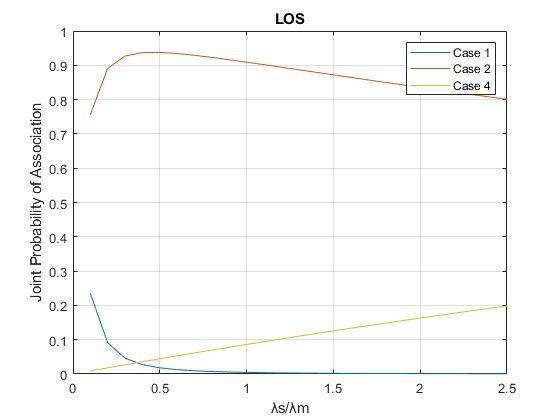
\includegraphics[scale=0.40]{jointprob_LOS.jpg}
\caption{\label{fig:our-p-LOS}Our Joint probability of association (LOS)}
\end{figure}

\begin{figure}[htbp]
\centering
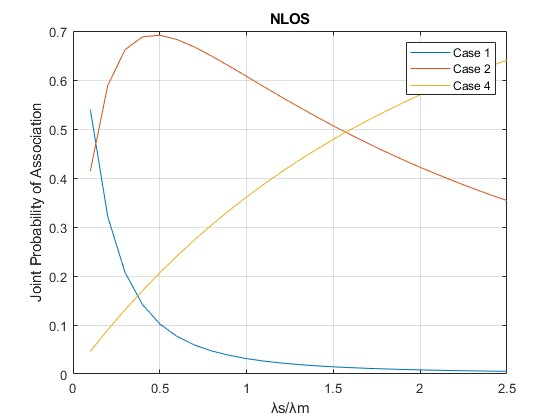
\includegraphics[scale=0.40]{jointprob_NLOS.jpg}
\caption{\label{fig:our-p-NLOS}Our Joint probability of association (NLOS)}
\end{figure}

\begin{figure}[htbp]
\centering
\includegraphics[scale=0.40]{SE_LOS_v2.jpg}
\caption{\label{fig:our-se-LOS}Our Spectral Efficiency Simulation(LOS)}
\end{figure}

\begin{figure}[htbp]
\centering
\includegraphics[scale=0.40]{SE_NLOS_v2.jpg}
\caption{\label{fig:our-se-NLOS}Our Spectral Efficiency Simulation(NLOS)}
\end{figure}

\subsection{Conclusion}
Our simulation results closely align with the results of the original paper, indicating that our modeling approach is correct.\par
The experiment presents that the line-of-sight (LOS) spectral efficiency have a significant improvement in the decoupled scenario. The original authors analyzed this phenomenon and attributed it to an increased proportion of small base stations (SBS) being used for uplink (UL) transmission. As the density of SBS increases, vehicles are closer to SBS, resulting in better UL power compared to macro base stations (MBS). Consequently, the increased proportion of SBS being used for UL transmission leads to a significant improvement in spectral efficiency.\par
In the future, we may considering applying this modeling approach to other application scenarios.

\begin{thebibliography}{00}
\bibitem{b1} Luofang Jiao, Kai Yu, Yunting Xu, Tianqi Zhang, Haibo Zhou, and Xuemin (Sherman) Shen.,"Spectral Efficiency Analysis of Uplink-Downlink
Decoupled Access in C-V2X Networks" in 2022 IEEE Global Communications Conference
\bibitem{b2} M. N. Sial, Y. Deng, J. Ahmed, A. Nallanathan and M. Dohler, "Stochastic Geometry Modeling of Cellular V2X Communication Over Shared Channels," in IEEE Transactions on Vehicular Technology, vol. 68, no. 12, pp. 11873-11887, Dec. 2019, doi: 10.1109/TVT.2019.2945481.
\bibitem{b3} Z. Sattar, J. V. Evangelista, G. Kaddoum, and N. Batani,
“Spectral efficiency analysis of the decoupled access
for downlink and uplink in two-tier network,” IEEE
Transactions on Vehicular Technology, vol. 68, no. 5, pp.
4871–4883, 2019.
\bibitem{b4} Chetlur, Vishnu Vardhan and Dhillon, Harpreet S, “Coverage
and rate analysis of downlink cellular vehicle-toeverything
(C-V2X) communication,” IEEE Transactions
on Wireless Communications, vol. 19, no. 3, pp. 1738–
1753, 2019.
\end{thebibliography}

\vspace{12pt}

\end{CJK*}
\end{document}
